\documentclass[a4paper,12 pt]{article}
\usepackage{geometry}
\geometry{letterpaper, margin=0.8in}
\usepackage[english]{babel}
\usepackage[utf8]{inputenc}
\usepackage{amsmath}
\usepackage{graphicx}
\usepackage{float}
\usepackage[numbered]{mcode}
\usepackage{indentfirst}
\renewcommand{\baselinestretch}{1.1}

\title{Using the Fourier Transform and Spectral Analysis to De-Noise Signal Data: A Canine Case Study}

\author{Dana Korssjoen} 

\date{24 January, 2020}

\begin{document}
\maketitle
\begin{abstract}
    This report applies Fast Fourier transform, spectral averaging, and spectral filtering to track an object's movement through fluid over time in a real world scenario. Discussion of theoretical foundations and algorithm implementation is included for all computational methods. The results of this report are precise coordinates for the object's location over time.
\end{abstract}
\section{Introduction and Overview}

Imagine, for a moment, a hypothetical scenario in which your dog (hypothetically named Fluffy) has swallowed a marble. Fearing for his canine life, you rush Fluffy to the vet, who uses ultrasound to obtain data on the spatial variations in the area of Fluffy's intestines where the marble is suspected to be. The vet intends to use this information to locate the marble's current position, so that he can focus an intense acoustic wave at that point to break it up. In a shocking turn of events, the vet inverts the business-client relationship, and asks you to analyze the highly noisy data to track the path of the marble. Fortunately, in this hypothetical scenario, you have read this lab report, so you are confident that you can track the marble.

This report will use the Fourier transform, spectral averaging, and spectral filtering to de-noise the data and compute the trajectory of the marble.

\section{Theoretical Background}
There are three major mathematical tools that I will be using to de-noise the data and track the marble over time: 1) Fourier transform, 2) spectral averaging, 3) and spectral filtering. In this section, I will describe the theoretical foundations for each of these techniques in detail.

\subsection{The Fourier Transform}

The Fourier transform is a mathematical technique that uses the Fourier series representation of a function to gain information about the underlying frequencies that compose it. If that doesn't sound familiar, recall that Fourier series take a given function and express it in terms of an infinite sum of sines and cosines (or, equivalently, complex exponentials). One major assumption here is that there \textit{are} underlying frequencies to be found in the function -- that is, that the data is periodic. The classical equations for the Fourier transform and its inverse, over the entire real line are
\begin{equation}
    F(k) = \frac{1}{\sqrt{2\pi}}\int_{-\infty}^{\infty}e^{-ikx}f(x)\:dx \quad\quad\quad f(x) = \frac{1}{\sqrt{2\pi}}\int_{-\infty}^{\infty} e^{ikx}F(k)\:dk.
\end{equation}

Note that these formulas are defined over the entire real line, which is an infinite domain. In practice, however, we are usually not interested in signals that started at the beginning of the universe and persist until the end of time, so we can take this transform over a finite domain, $x\in[-L,L]$ for some real $L$. Working in a discrete domain like this, the Fourier transform gives us a finite expansion of our original function in terms of sines and cosines (or complex exponentials), over which we can integrate. We end up with a transformed signal in frequency space, which enables us to easily analyze the relative occurrence of different frequencies within the signal. Once in frequency space, we can either use an inverse transform to go back to the domain occupied by the original signal, or to apply the frequency-based computational techniques described below.

In practice, the Fourier transform is implemented computationally using the Fast Fourier transform algorithm, which has the advantages of a low operation count ($O(N\log N)$) and excellent accuracy compared to other discretization schemes.

\subsection{Spectral Averaging}
Spectral averaging is a common method of reducing noise and increasing time-frequency resolution in a signal. The method is pretty straightforward - if you have multiple readings from the same object of interest over time, take the average of these signals in frequency space to hopefully cancel out noise. In order for this to work, a couple of assumptions must be met: i) the frequency of interest is relatively constant over time (otherwise, averaging will reduce frequency resolution), ii) you have multiple readings from that object (or else you can't average), and iii) the noise in your measurements has zero mean. This last point is true for white noise, which is distributed normally. For this reason, spectral averaging is a strong tactic for de-noising recurring signals like radars. An important precaution to take before using spectral averaging, however, is to \textit{make sure} that you're operating in frequency space, not time space, because your object may be moving over time.

\subsection{Spectral Filtering}
As the name implies, spectral filtering is the practice of filtering a signal to extract information at certain desired frequencies. The basic idea is to determine the frequency of interest, then center the filter around it to amplify signals at or around that frequency, and minimize those at different frequencies. In order to do this, the signal must be expressed in frequency space, so a technique like the Fourier transform is a necessary first step. 

There are many different filters to choose from, but all of them intend to accomplish the basic idea described here: amplify the frequency of interest, and minimize interference from unrelated signals. One of the simplest choices for a filter is the Gaussian (or the normal distribution, for my statistician friends).

With that background established, let's move on the de-noising the signal in question.

\section{Algorithm Implementation and Development}
\subsection{Initialize Important Variables: Lines 1-16}
In this section, we load the data and initialize the variables we'll need for the analysis. In particular, we choose $L$, which determines the size of our spatial window, and $n$, which is our number of Fourier modes, i.e. we have $2^n$ data points. Note that the number of data points \textit{must} be some power of $2$ for this method to work as expected. In this case, $L=15$ and $n=64$.

The rest of the initialization here is for axes. We will analyze over $n$ equally spaced points between $-L$ (inclusive) and $L$ (exclusive) in the spatial domain to match the dimensions of our data. In the frequency domain,  the number of points we have is determined by our Fourier mode, $n=64$, and we rescale it by $2\pi/L$ because the Fast Fourier transform assumes that our signals have a periodicity of $2\pi$ (as do the sine and cosine functions).  Finally, we have to shift our frequency vector with \textbf{fftshift()} to put the zero-frequency component in the center of the vector, which aligns with the output we'll get from \textbf{fftn()}. We make a meshgrid of this vector to get our wavenumber matrices.

\subsection{Spectral Averaging: Lines 17-30}
In this section, we loop over the 20 measurements we have recorded, reshaping each one into a $n\times n\times n$ matrix, since it was saved in flattened form, then we take the Fast Fourier transform of that measurement and add it to our running average. At the end, we take the absolute value (to handle complex values) and divide by the number of measurements. For more on why this was done, see section 2.2. Code for plotting the averaged signal is included on lines 26-29, though the data is still very noisy. 

\subsection{Filtering: Lines 31-56}
The first step in building the filter is finding the frequency signature of the marble, which is why we averaged out (some of) the noise first. Remember that we are operating in frequency space here, so the position of the maximum value in the matrix corresponds to the center frequency, also called the frequency signature. We look at that position in the wavenumber matrices that we generated before to find the wavenumber for each dimension.

We build the filter out of a Gaussian distribution based on the frequency signature. The choice of $\tau$ was after some experimentation (it determines the width of the filter).

Finally, we apply our filter by taking the FFT of our reshaped data, multiplying it with the filter to amplify the marble's frequency signature, and taking the inverse FFT to get back into the spatial domain. The marble should now be outputting the most dominant signal in the data, so we find the maximum reading of each of the 20 measurements to track the marble's location over time.

\subsection{Plot Trajectory: Lines 57-66}
This section simply contains the code to track the path of the marble through Fluffy's intestines. You can use the code to generate it yourself, or else you can just look at Figure 1 in the next section.

\section{Computational Results}
Having finally finished de-noising the data, determining the frequency signature of the marble, filtering the data, and tracking the marble's trajectory, we can now say that the marble's frequency signature was $(k_x, k_y, k_z) = (-4.8171, 5.6549, -6.7021)$. We used this to plot its path through Fluffy's intestines. You can see it for yourself in Figure 1. In the figure, the large red dot represents the position of the marble at the 20th measurement. It is at approximately $(x,y,z)=(-5.6250, 4.2188, -6.0938)$. The full table of positions in included in this section as Table 1. 

With this information obtained, we are ready to report to the vet and save Fluffy from this lethal marble.
 
\vspace{10mm}
\begin{figure}[H]
  \centering
    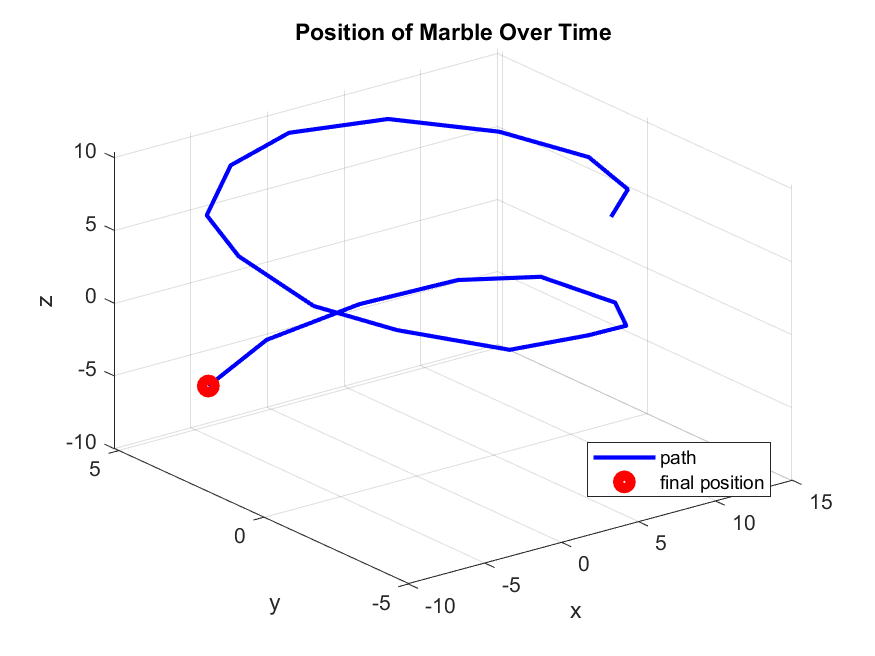
\includegraphics[width = 0.7\textwidth]{hw1/images/MarblePath.png}
    \label{fig:example}
\caption{The path of the marble}
\end{figure}

\begin{table}[H]
\centering
\begin{tabular}{|l|l|l|l|}
\hline
Measurement & x position & y position & z position \\ \hline
1          & 4.6875  & -4.2188 & 10.3125 \\ \hline
2          & 8.4375  & -2.8125 & 9.8438  \\ \hline
3          & 10.3125 & -0.4688 & 9.3750  \\ \hline
4          & 8.9063  & 1.8750  & 9.3750  \\ \hline
5          & 6.0938  & 4.2188  & 8.9063  \\ \hline
6          & 1.4073  & 5.1563  & 8.4375  \\ \hline
7          & -3.2813 & 4.6875  & 7.9688  \\ \hline
8          & -7.5000 & 3.2813  & 7.0313  \\ \hline
9          & -9.8438 & 0.9375  & 7.0313  \\ \hline
10         & -9.3750 & -1.4063 & 5.6250  \\ \hline
11         & -7.5000 & -3.2813 & 5.1563  \\ \hline
12         & -2.8125 & -4.6875 & 3.7500  \\ \hline
13         & 2.3438  & -4.6875 & 3.2813  \\ \hline
14         & 6.5625  & -3.7500 & 1.8750  \\ \hline
15         & 9.3750  & -1.8750 & 0.9375  \\ \hline
16         & 9.8438  & 0.9375  & 0       \\ \hline
17         & 7.9688  & 2.8125  & -1.4063 \\ \hline
18         & 4.2188  & 4.2188  & -3.2813 \\ \hline
19         & -0.9375 & 4.6875  & -4.6875 \\ \hline
20         & -5.6250 & 4.2188  & -6.0938 \\ \hline
\end{tabular}
\caption{Marble's position over time}
\end{table}

\section{Summary and Conclusions}
The Fast Fourier transform is an efficient computational method to extract information about the frequency composition of a periodic signal. In this report, it was combined with spectral averaging and spectral filtering, which are both powerful methods of de-noising frequency data while preserving information about the signal of interest. These computational methods are literally live-saving -- in fact, they saved the life of your (hypothetical) dog, Fluffy.


\section{Appendix A: MATLAB Glossary}
Commands are listed in the order that they are first used.

\textbf{linspace(a,b,n)}: returns a vector with $n$ points linearly spaced between $a$ and $b$.

\textbf{fftshift(A)}: shifts the zero-frequency component of $A$ to the center of $A$.

\textbf{meshgrid(x,y,z)}: returns 3-D grid coordinates defined by the $x, y$, and $z$ vectors.

\textbf{zeros(n,n,n)}: returns a zero matrix of the specified size.

\textbf{reshape(A,sz)}: reshapes $A$ into a matrix of the size specified by $sz$.

\textbf{fftn(A)}: performs a multidimensional Fast Fourier transform of matrix $A$.

\textbf{abs(A)}: takes the absolute value of every element in $A$.

\textbf{isosurface(X,Y,Z,V,isovalue)}: returns an isosurface plot of volume data $V$ which connects points with the specified isovalue, and has axes specified by $X,Y,$ and $Z$, 

\textbf{median(A,'all')}: finds the median value in multidimensional matrix $A$.

\textbf{[val,ind]=max(A)}: returns the maximum value (val) of $A$ and the index (ind) at which it occurs.

\textbf{[i,j,k]=ind2sub([n,n,n],ind)}: converts a linear index to subscripts in a multidimensional matrix with specified size.

\textbf{exp(n)}: represents the mathematical function $e^n$.

\textbf{ifftn(A)}: performs the multidimensional inverse Fast Fourier transform of $A$.

\textbf{plot3()}: plot in 3 dimensions, as in figure 1.

\section{Appendix B: MATLAB Code}
Below is the body of the code necessary to compute these results.
\begin{lstlisting}
%% initialize important variables
clear; close all; clc;
load Testdata

L=15; % spatial domain
n=64; % Fourier modes
x2=linspace(-L,L,n+1);
x=x2(1:n);
y=x;
z=x;
k=(2*pi/(2*L))*[0:(n/2-1) -n/2:-1]; % rescale frequencies
ks=fftshift(k);

[X,Y,Z]=meshgrid(x,y,z);
[Kx,Ky,Kz]=meshgrid(ks,ks,ks);

%% spectral averaging
ave=zeros(n,n,n);
for j=1:20
    Un(:,:,:)=reshape(Undata(j,:),n,n,n);
    Unfft=fftn(Un);
    ave=ave+Unfft;
end
ave=abs(ave)/20;

% plot if desired - data is very messy, though
close all;
isosurface(Kx,Ky,Kz,fftshift(ave),median(abs(ave),'all'));
axis([-7 7 -7 7 -7 7]), grid on

%% filtering
% find frequency signature
[val,ind]=max(ave(:));
[i,j,k]=ind2sub([n,n,n],ind);
kx0=Kx(i,j,k);
ky0=Ky(i,j,k);
kz0=Kz(i,j,k);

% build filter
tau = 1; % width of filter
mfilter = exp(-tau*((Kx-kx0).^2+(Ky-ky0).^2+(Kz-kz0).^2));

% find dominant signal component at each time step
xpos=zeros(1,20);
ypos=zeros(1,20);
zpos=zeros(1,20);
for j = 1:20
    Un(:,:,:)=reshape(Undata(j,:),n,n,n);
    Ufiltered = ifftn(fftn(Un).*mfilter);
    [val,ind]=max(Ufiltered(:)); 
    [xm,ym,zm]=ind2sub([n,n,n],ind);
    xpos(j)=X(xm,ym,zm); 
    ypos(j)=Y(xm,ym,zm);
    zpos(j)=Z(xm,ym,zm);
end

%% plot trajectory
plot3(xpos,ypos,zpos,'b','Linewidth',2);
grid on, hold on
% highlight final position
plot3(xpos(end),ypos(end),zpos(end),'ro','Linewidth',5);
xlabel('x')
ylabel('y')
zlabel('z')
legend({'path','final position'},'Location','Best');
title('Position of Marble Over Time')
\end{lstlisting}
\end{document}